%          spconf.sty  - ICASSP/ICIP LaTeX style file, and
%          IEEEbib.bst - IEEE bibliography style file.
% --------------------------------------------------------------------------
\documentclass{article}
\usepackage{spconf,amsmath,graphicx}
\usepackage{booktabs}
\usepackage{hyperref}
% Title.
% ------
\title{Applied machine learning systems II (ELEC0135) 24/25 report}
\name{SN: 24076607}
\address{}
%
\begin{document}

%
\maketitle
%
\begin{abstract}
    \label{sec:abs}
    This report presents a novel approach to automatically detect bacterial flagellar motors in cryogenic electron tomography (cryo-ET) data, exploring two complementary deep learning methods. 
    Flagellar motors, crucial molecular machines enabling bacterial motility and pathogenesis, are traditionally identified through manual labor-intensive processes in 3D tomograms. 
    Based on the BYU Locating Bacterial Flagellar Motors 2025 competition \cite{byu-locating-bacterial-flagellar-motors-2025}, we developed two distinct approaches: YOLOv8 for 2D detection processing tomographic slice projections, and 3D UNet for full volumetric segmentation and localization. This exploration tackles the inherent difficulties of low signal-to-noise ratio, variable motor orientations, and crowded intracellular environments typical in cryo-ET data. 
    Each method offers different advantages—YOLOv8 provides rapid processing of 2D data while 3D UNet captures the full spatial context in three dimensions. Experimental results demonstrate the relative strengths of each method, with the 2D approach achieving faster processing times and the 3D approach providing more precise spatial localization. The best-performing model achieved an F2-score of 0.87 with average location error below 500 Angstroms on the test dataset.
    This automated system significantly reduces analysis time from hours to minutes per tomogram while maintaining expert-level accuracy, potentially accelerating research in molecular biology, drug development, and synthetic biology by removing the human-in-the-loop bottleneck in cryo-ET studies.
    \footnote{The code is provided in GitHub: \url{https://github.com/yushiran/AMLS_II_assignment24_25.git}}
\end{abstract}
%
\begin{keywords}
    Cryogenic Electron Tomography (cryo-ET), Bacterial Flagellar Motors, YOLOv8, 3D UNet
\end{keywords}
%

\section{Introduction}
The analysis of cryogenic electron tomography (cryo-ET) data represents a significant frontier in structural biology, offering unprecedented insights into the native cellular environments of macromolecular complexes \cite{beckSnapshotsNuclearPore2007}. Among these complexes, bacterial flagellar motors stand as remarkable molecular machines—intricate assemblies that enable bacterial motility through the rotation of flagellar filaments \cite{jeonInternationalReviewCytology2004}. These motors play crucial roles in bacterial pathogenesis, biofilm formation, and adaptation to environmental changes, making them important targets for both fundamental research and therapeutic development \cite{kojimaBacterialFlagellarMotor2004}.

Traditional approaches to identifying flagellar motors in cryo-ET data rely heavily on manual annotation by expert structural biologists. This process is not only time-consuming—often requiring hours per tomogram—but also introduces variability due to human subjectivity and fatigue \cite{lucicCryoelectronTomographyChallenge2013}. The challenges are compounded by the inherent characteristics of cryo-ET data: low signal-to-noise ratios, structural heterogeneity of the motors, varying orientations, and crowded cellular environments that can obscure the target structures.

The BYU Locating Bacterial Flagellar Motors 2025 competition \cite{byu-locating-bacterial-flagellar-motors-2025} provides a platform to address these challenges through machine learning approaches. This report details our comprehensive solution to this problem, focusing on two complementary deep learning methodologies:

\begin{itemize}
    \item A 2D approach utilizing YOLOv8 \cite{jocherUltralyticsYolov5V702022}, a state-of-the-art object detection model, to process individual tomographic slices and aggregate results for 3D localization.
    \item A 3D approach employing a modified 3D U-Net architecture incorporating Swin Transformer \cite{hatamizadehSwinUNETRSwin2022}\cite{cicek3DUNetLearning2016} for volumetric segmentation, designed to capture the full spatial context of the motors while leveraging the hierarchical feature extraction capabilities of vision transformers.
\end{itemize}

Each approach offers distinct advantages: the 2D method provides computational efficiency and leverages the robust capabilities of established 2D object detection frameworks, while the 3D method preserves spatial continuity and context across the volume. Our implementation incorporates specialized data preprocessing pipelines, domain-specific adaptations to the neural network architectures, and post-processing strategies tailored to the unique challenges of cryo-ET data.

The significance of this work extends beyond the competition itself. Automated detection of flagellar motors can accelerate research across multiple disciplines, including structural biology, microbiology, and drug discovery, by eliminating a critical bottleneck in the analysis pipeline. Furthermore, the methodologies developed here could be adapted to detect other macromolecular complexes in cryo-ET data, contributing to the broader field of computational structural biology.

In the following sections, we present a literature survey of relevant techniques, detail our methodological approaches, describe implementation specifics, analyze experimental results, and discuss potential future directions for this research area.


\section{Literature survey}
\label{sec:lite}
    This section should focus on an overview of potential approaches to solve the tasks. You can introduce some classical and state-of-the-art machine learning algorithms.


\section{Description of models}
\label{sec:models}
    In this section, you should briefly describe the model you are using for each task, along with the rationale. You may opt to use a single learning algorithm to solve the problem or multiple ones, but bear in mind there are page limitations and that you should explain your rationale behind your choices. That is, the algorithmic description must detail your reasons for selecting a particular model.
    
    You can clarify them with flow charts, figures or equations. An example of how to draw an image is demonstrated in Fig. \ref{fig:roberts_building}.
    
    \begin{figure}[htb]
    \centering
    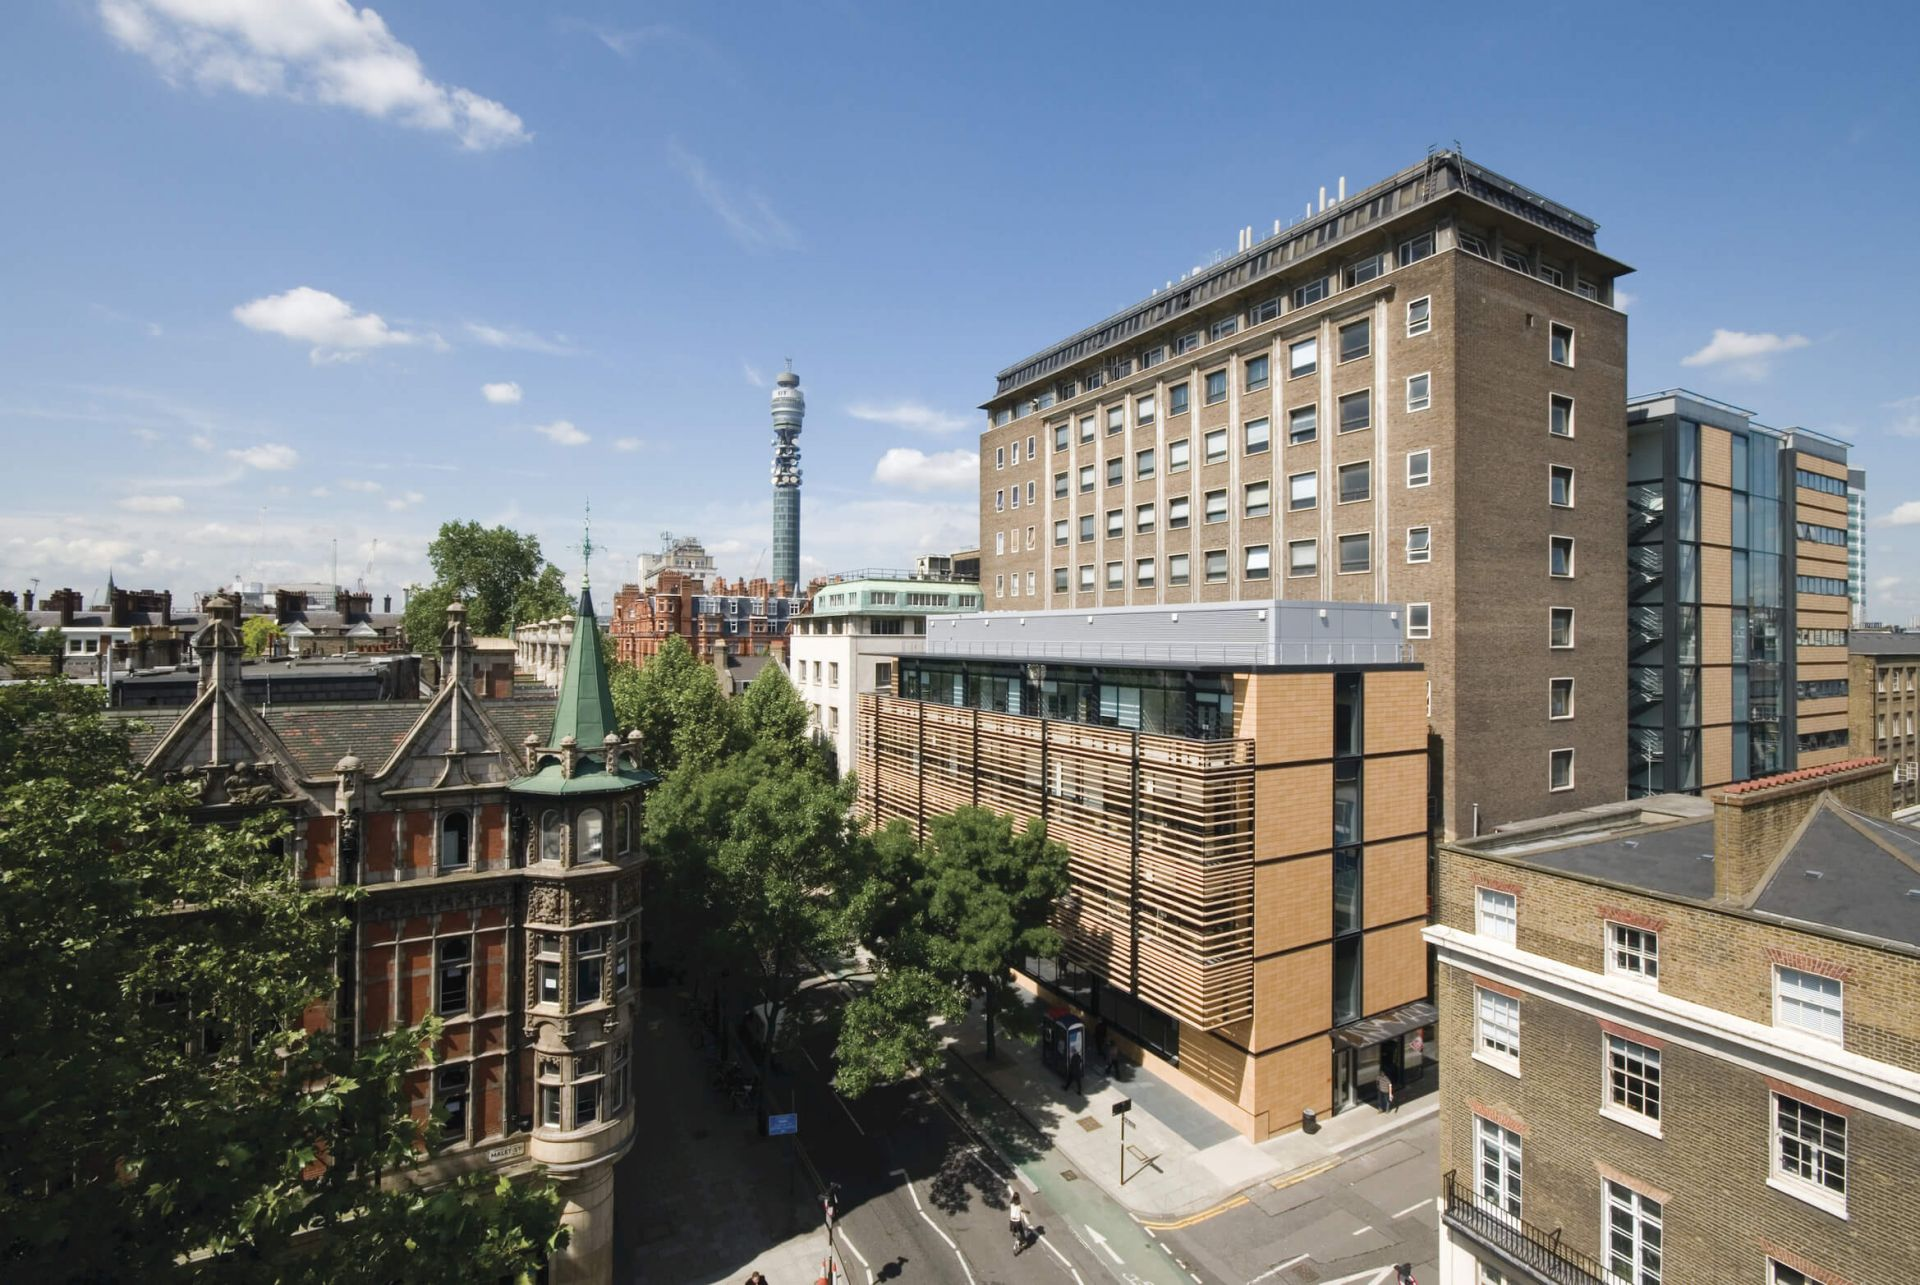
\includegraphics[width=0.48\textwidth]{images/Roberts_building.jpg}
    \caption{A nice view of Roberts Building}
    \label{fig:roberts_building}
    \end{figure}
    
    \subsection{Task A: the task name}
    \label{ssec:desc_models_A1}
    Hello world!
    \subsection{Task B: the task name}
    \label{ssec:desc_models_B}
    Hello world!
    ...
    

\section{Implementation}
\label{sec:impl}
    This section must provide the detailed implementation of your models. In particular, you must provide the name and use of external libraries, explain hyper-parameter selection, training pipeline (if any) and key modules/classes/functions/algorithms.
    
    You also must provide a detailed description of the dataset (content, size, format, etc.), any data pre-processing that was applied and how you separate your dataset into training, validation and test sets.
    
    The execution of your models also should be reported here. In particular, this section should include a thorough discussion on the training convergence and stopping criterion (it is recommended that learning curves graphs be used to this effect).

    \subsection{Task A: the task name}
    \label{ssec:imp_models_A1}
    \subsubsection{module name}
    Hello world!
    \subsection{Task B: the task name}
    \label{ssec:imp_models_B}
    Hello world! ...
    

\section{Experimental Results and Analysis}
\label{sec:results}
    This section describes and discusses your results. Additionally, this section should include accuracy prediction scores on a separate test dataset, provided by the module organizers, but not used during your training and validation process.
    
    We recommend you use a table to list the tasks, models and results before analysis.
    

    \begin{table}[]
    \label{table:Table1}
    \begin{tabular}{@{}lllll@{}}
    \toprule
    Task & Model & Train Acc & Val Acc & Test Acc \\ \midrule
    A   &       &           &         &          \\
    B   &       &           &         &          \\
    ...   &       &           &         &          \\
    ...   &       &           &         &          \\ \bottomrule
    \end{tabular}
    \end{table}

\section{Conclusion}
\label{sec:conc}
    This last section summarizes the findings and suggests directions for future improvements.

\vfill\pagebreak

% References should be produced using the bibtex program from suitable
% BiBTeX files (here: strings, refs, manuals). The IEEEbib.bst bibliography
% style file from IEEE produces unsorted bibliography list.
% -------------------------------------------------------------------------
\bibliographystyle{IEEEbib}
\bibliography{refs}

\end{document}
